%%%%%%%%%%%%%%%%%%%%%%%%%%%%%%%%%%%%%%%%%%%%%%%%%%%%%%%%%%%%
%%  This Beamer template was created by Cameron Bracken.
%%  Anyone can freely use or modify it for any purpose
%%  without attribution.
%%
%%  Last Modified: January 9, 2009
%%

\documentclass[xcolor=x11names,compress]{beamer}

%% General document %%%%%%%%%%%%%%%%%%%%%%%%%%%%%%%%%%
\usepackage{graphicx}
\usepackage{pgfplots}
\usepackage{tikz}
\usepackage{siunitx}
\usepackage{tikz}
\usetikzlibrary{arrows,automata}
\usepackage{siunitx}
\usepackage{pgf}
\usetikzlibrary{arrows}
\usetikzlibrary{decorations.fractals, arrows}
\usetikzlibrary{arrows,decorations.pathreplacing}
%%%%%%%%%%%%%%%%%%%%%%%%%%%%%%%%%%%%%%%%%%%%%%%%%%%%%%


%% Beamer Layout %%%%%%%%%%%%%%%%%%%%%%%%%%%%%%%%%%
\useoutertheme[subsection=false,shadow]{miniframes}
\useinnertheme{default}
\usefonttheme{serif}
\usepackage{palatino}

\setbeamerfont{title like}{shape=\scshape}
\setbeamerfont{frametitle}{shape=\scshape}

\setbeamercolor*{lower separation line head}{bg=DeepSkyBlue4}
\setbeamercolor*{normal text}{fg=black,bg=white}
\setbeamercolor*{alerted text}{fg=red}
\setbeamercolor*{example text}{fg=black}
\setbeamercolor*{structure}{fg=black}

\setbeamercolor*{palette tertiary}{fg=black,bg=black!10}
\setbeamercolor*{palette quaternary}{fg=black,bg=black!10}

\renewcommand{\(}{\begin{columns}}
\renewcommand{\)}{\end{columns}}
\newcommand{\<}[1]{\begin{column}{#1}}
\renewcommand{\>}{\end{column}}
%%%%%%%%%%%%%%%%%%%%%%%%%%%%%%%%%%%%%%%%%%%%%%%%%%




\begin{document}


%%%%%%%%%%%%%%%%%%%%%%%%%%%%%%%%%%%%%%%%%%%%%%%%%%%%%%
%%%%%%%%%%%%%%%%%%%%%%%%%%%%%%%%%%%%%%%%%%%%%%%%%%%%%%
\section{\scshape Introduction}
\begin{frame}
\title{Presentation Title}
%\subtitle{SUBTITLE}
\author{
	Cameron Bracken\\
	{\it Humboldt State University}\\
}
\date{
	\begin{tikzpicture}[decoration=Koch curve type 2]
		\draw[DeepSkyBlue4] decorate{ decorate{ decorate{ (0,0) -- (3,0) }}};
	\end{tikzpicture}
	\\
	\vspace{1cm}
	\today
}
\titlepage
\end{frame}

\begin{frame}{Introduction}
\tableofcontents
\end{frame}



\begin{frame}
\title{\huge Time-optimised Route Planning for Electric Vehicles}
%\subtitle{SUBTITLE}
\author{
 Simon Buus Jensen,\\
 Andreas Berre Eriksen,\\
 Mikkel Alexander Madsen,\\
 Mathias Meldgaard Andersen\\
}
\titlepage
\end{frame}

\begin{frame}{Table of Contents}
\tableofcontents
\end{frame}

\section{\scshape Introduction}
\subsection{Motivation}
\begin{frame}{Motivation}
\begin{itemize}
\item Why is route planning for EVs an interesting problem?
\end{itemize}
\begin{figure}[h!]
  \centering
  Plug-in Vehicle production
    \includegraphics[height=0.5\textwidth]{images/forecast}
  
      \tiny Credit: IHS automotive
\end{figure}
\end{frame}

\begin{frame}{Motivation}
\begin{itemize}
\item Why is route planning for EVs an interesting problem?
\end{itemize}
\begin{figure}[h!]
  \centering
  Fast-charging stations worldwide
    \includegraphics[height=0.5\textwidth]{images/forecast2}
  
      \tiny Credit: IHS automotive
\end{figure}
\end{frame}

\section{Greedy Heuristic Algorithm}

\begin{frame}{Example}
    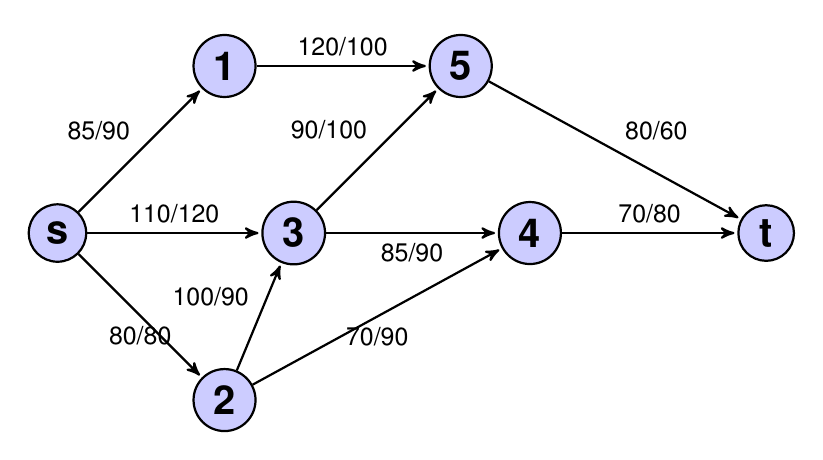
\begin{tikzpicture}[->,>=stealth',shorten >=1pt,auto,node distance=3cm,
  thick,main node/.style={circle,fill=blue!20,draw,font=\sffamily\Large\bfseries}]

  \node[main node] (s) {s};
  \node[main node] (1) [above right of=s] {1};
  \node[main node] (2) [below right of=s] {2};
  \node[main node] (3) [right of=s] {3};
  \node[main node] (4) [right of=3] {4};
  \node[main node] (5) [right of=1] {5};
  \node[main node] (t) [right of=4] {t};


  \path[every node/.style={font=\sffamily\small}]
      (s) edge node {85/90} (1)
      (s) edge node [below] {80/80} (2)
      (s) edge node {110/120} (3)

      (1) edge node {120/100} (5)

      (2) edge node {100/90} (3)
      (2) edge node [below] {70/90} (4)

      (3) edge node [below] {85/90} (4)
      (3) edge node {90/100} (5)

      (4) edge node {70/80} (t)

      (5) edge node {80/60} (t);
\end{tikzpicture}

\end{frame}

\section{Optimal solution to a path}
\subsection{Modeling of the physical system}
\begin{frame}{Physical system}
Modeling the physical system, of an EV and a path.
\begin{figure}[!htb]
\centering
    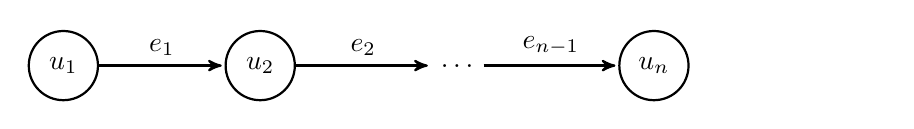
\begin{tikzpicture}[shorten >=1pt,node distance=2.5cm,>=stealth',thick]
        \node[state] (1) {$u_1$};
        \node[state] (2) [right of=1] {$u_2$};
        \node[] (dots) [right of=2] {$\dots$};
        \node[state] (n) [right of=dots] {$u_n$};
        \node[state,draw=none] (d1) [right of=n] {};
        \draw [->] (1) to[right] node[auto] {$e_1$} (2);
        \draw [->] (2) to[right] node[auto] {$e_2$} (dots);
        \draw [->] (dots) to[right] node[auto] {$e_{n-1}$} (n);
        %\draw [->] (n) to[right] node[auto] {$e_n$} (d1);
    \end{tikzpicture}
\end{figure} 
\begin{itemize}
\item Path
\begin{itemize}
\item[+] Charging stations, with charging rate ($R_{CH}(u_i)$)
\item[+] Road segments, with speed limit ($v_{min}(e_i)$, $v_{max}(e_i)$) and distance ($D(e_i)$) 
\end{itemize}
\item EV
\begin{itemize}
\item[+] Driving consumes energy accordingly to the speed of the EV, defined by: ($R_{CO}(e_i)$)
\item[+] Further two constants from the EV are important to model, namely, battery capacity ($B_{max}$) and initial battery ($B_{cur}$)
\end{itemize}
\end{itemize} 
\end{frame}
\subsection{Optimisation problem}
\begin{frame}{Optimisation problem}
Formulating a optimisation problem, which when solved will yield a optimal solution. 
\begin{itemize}
\item Objective: Move from $u_1$ to $u_n$ using minimum time . 
\begin{itemize}
\item[+] Time can be used driving or charging. 
\begin{itemize}
\item[-] $\text{min: } \sum_{i=1}^{n-1} \left(\frac{D(e_i)}{v_{e_i}} + CT_{u_i} \right)$
\end{itemize}
\end{itemize}
\item Physical constraints:
\begin{itemize}
\item[+] Each edge must be driven at a speed within the speed limit:\begin{itemize}
\item [-] $\forall_{i\in1 \dots n-1 }:\;v_{min}(e_i) \leq v_{e_i} \leq v_{max}(e_i)$
\end{itemize}
\item[+] Time can only be positive.\begin{itemize}
\item [-] $\forall_{i\in1 \dots n }:\; 0 \leq CT_{u_i} $
\end{itemize}

\item[+] The energy is the battery must alway be between 0 and $B_{max}$
\end{itemize}
\end{itemize} 
\end{frame}
\begin{frame}{battery constraint}
The battery constraint of the optimisation problem can be split into two parts
\begin{itemize}
\item No road segment can be passed without having the required energy
\item No overcharging at any charging station. 
\end{itemize}
Energy can be..
\begin{itemize}
\item Spend: $\forall_{i\in1 \dots n-1 }:\; ES(e_i) = D(e_i) \times R_{CO}(v_{e_i})$
\item Acuried: $\forall_{i\in1 \dots n }:\; EA(u_i) = R_{CH}(u_i) \times CT_{u_i}$
\item Already in the battery: $B_{cur}$
\end{itemize}
\end{frame}
\begin{frame}{battery constraint}
No road segment can be passed without having the required energy 
\begin{figure}[!htb]
\centering
    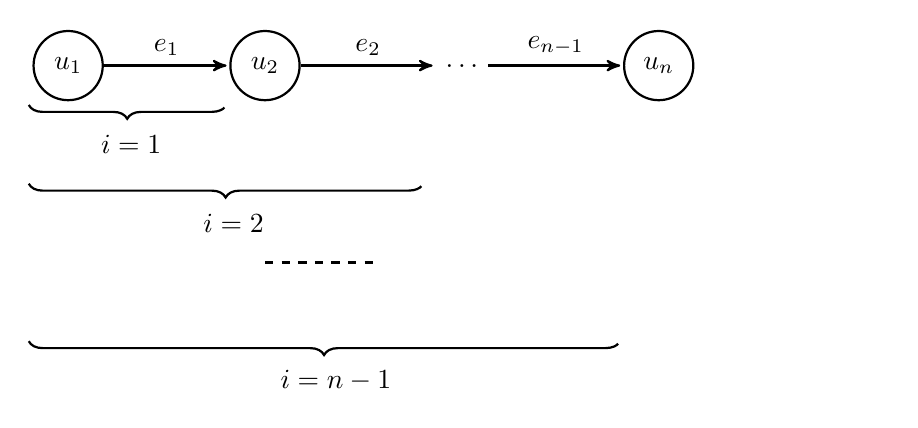
\begin{tikzpicture}[shorten >=1pt,node distance=2.5cm,>=stealth',thick]
        \node[state] (1) {$u_1$};
        \node[state] (2) [right of=1] {$u_2$};
        \node[] (dots) [right of=2] {$\dots$};
        \node[state] (n) [right of=dots] {$u_n$};
        \node[state,draw=none] (d1) [right of=n] {};
        \draw [->] (1) to[right] node[auto] {$e_1$} (2);
        \draw [->] (2) to[right] node[auto] {$e_2$} (dots);
        \draw [->] (dots) to[right] node[auto] {$e_{n-1}$} (n);
        %\draw [->] (n) to[right] node[auto] {$e_n$} (d1);
        \draw[decorate,decoration={brace,amplitude=5pt,mirror}] 
    (-0.5,-0.5) coordinate (1) -- (2,-0.5) coordinate (2);
    \node at (0.8,-1.0){$i=1$};
     \draw[decorate,decoration={brace,amplitude=5pt,mirror}] 
    (-0.5,-1.5) coordinate (1) -- (4.5,-1.5) coordinate (2);
    \node at (2.1,-2.0){$i=2$};
    \draw [dashed] (2.5,-2.5) -- (4,-2.5);
     \draw[decorate,decoration={brace,amplitude=5pt,mirror}] 
    (-0.5,-3.5) coordinate (1) -- (7,-3.5) coordinate (2);
    \node at (3.4,-4.0){$i=n-1$};

    \end{tikzpicture}
\end{figure} 
\begin{itemize}
\item $\forall_{i\in1 \dots n-1 }:\;0 \leq B_{cur} + \sum_{j=1}^{i} EA(u_j) - \sum_{j=1}^{i} ES(e_j) \leq B_{max}$
\end{itemize}
\end{frame}

\begin{frame}{battery constraint}
No overcharging at any charging station.
\begin{figure}[!htb]
\centering
    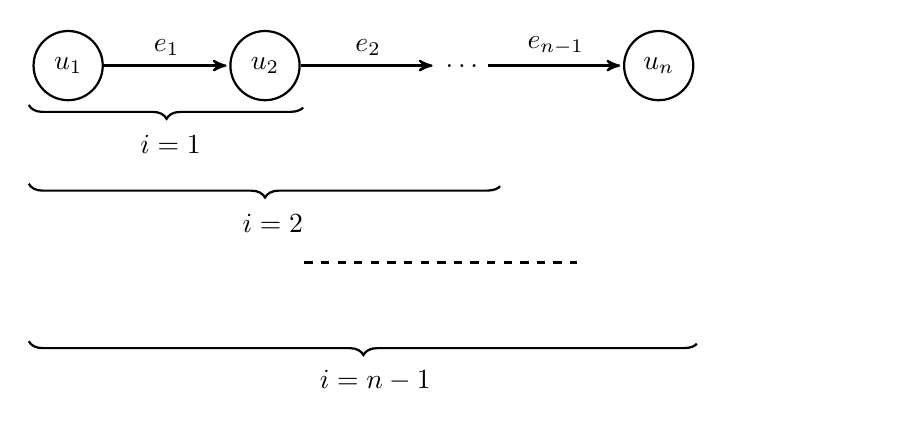
\begin{tikzpicture}[shorten >=1pt,node distance=2.5cm,>=stealth',thick]
        \node[state] (1) {$u_1$};
        \node[state] (2) [right of=1] {$u_2$};
        \node[] (dots) [right of=2] {$\dots$};
        \node[state] (n) [right of=dots] {$u_n$};
        \node[state,draw=none] (d1) [right of=n] {};
        \draw [->] (1) to[right] node[auto] {$e_1$} (2);
        \draw [->] (2) to[right] node[auto] {$e_2$} (dots);
        \draw [->] (dots) to[right] node[auto] {$e_{n-1}$} (n);
        %\draw [->] (n) to[right] node[auto] {$e_n$} (d1);
        \draw[decorate,decoration={brace,amplitude=5pt,mirror}] 
    (-0.5,-0.5) coordinate (1) -- (3,-0.5) coordinate (2);
    \node at (1.3,-1.0){$i=1$};
     \draw[decorate,decoration={brace,amplitude=5pt,mirror}] 
    (-0.5,-1.5) coordinate (1) -- (5.5,-1.5) coordinate (2);
    \node at (2.6,-2.0){$i=2$};
    \draw [dashed] (3,-2.5) -- (6.5,-2.5);
     \draw[decorate,decoration={brace,amplitude=5pt,mirror}] 
    (-0.5,-3.5) coordinate (1) -- (8,-3.5) coordinate (2);
    \node at (3.9,-4.0){$i=n-1$};

    \end{tikzpicture}
\end{figure} 
\begin{itemize}
\item $\forall_{i\in1 \dots n-1}:\;0 \leq B_{cur} + \sum_{j=1}^{i+1} EA(u_j) - \sum_{j=1}^{i} ES(e_j) \leq B_{max}$
\end{itemize}
\end{frame}
\subsection{Linear programming}
\begin{frame}{Linear programming}
NP-complete problem.

Linearization and linear programming for approximate solution. 

Two functions of the optimisation problem are non linear functions. 
\begin{itemize}
\item Consumption rate ($R_{CO}(v_{e_i})$)
\item Driving time ($\frac{D(e_i)}{v_{e_i}}$)
\end{itemize}
\end{frame}


\begin{frame}{linearization example}
Function for energy consumption before linearization. $R_{CO}(v)=0.019*x^2 - 0.770*x + 184.4$
\begin{figure}[!htb]
\label{fig:graph}
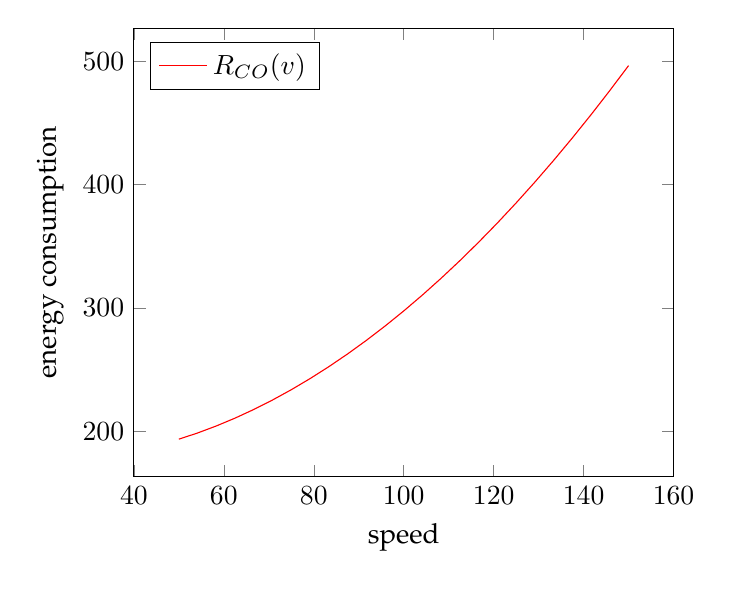
\begin{tikzpicture}
\begin{axis}[xlabel=speed, ylabel=energy consumption,legend style={legend pos=north west}]
\addplot[draw=red,domain=50:150]{(0.019*x^2 - 0.770*x + 184.49) };
\addlegendentry{$R_{CO}(v)$}

% \addplot[mark=*, domain=25:75] coordinates {(37,295)};
\end{axis}
\end{tikzpicture}% 

\label{fig:graph}
\end{figure}
\end{frame}

\begin{frame}{linearization example}
Function for energy consumption after linearization. $R_{CO}(v)=0.019*x^2 - 0.770*x + 184.4$
\begin{figure}[!htb]
\label{fig:graph}
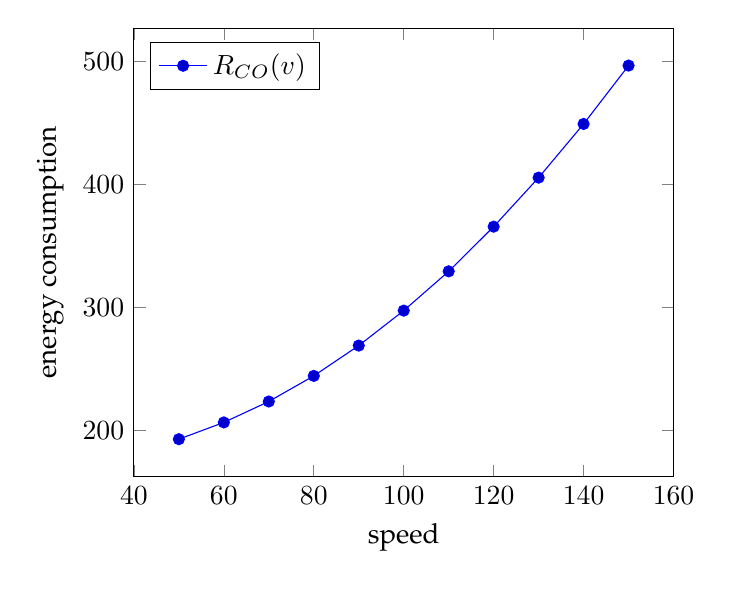
\begin{tikzpicture}
\begin{axis}[xlabel=speed, ylabel=energy consumption,legend style={legend pos=north west}]
\addplot coordinates { (50,193) (60,206.6) (70,223.6) (80,244.4) (90,269) (100,297.4) (110,329.3) (120,365.6) (130,405.4) (140, 449) (150,496.4) }; \addlegendentry{$R_{CO}(v)$ }

% \addplot[mark=*, domain=25:75] coordinates {(37,295)};
\end{axis}
\end{tikzpicture}% 

\label{fig:graph}
\end{figure}
\begin{itemize}
\item For all linear function their slope and the y-intercept is precomputed. 
\item For every edge in the path exactly one line segment needs to be chosen. Thus a binary matrix i introduced of size $n \times m$, where $n$ is edges in the path and $m$ is linear pieces of each line. 
\end{itemize}
\end{frame}
\begin{frame}{linearization example}
\begin{itemize}
\item For all linear function their slope and the y-intercept is precomputed. 
\item For every edge in the path exactly one line segment needs to be chosen. Thus a binary matrix i introduced of size $n \times m$, where $n=$edges in the path and $m=$linear pieces of each line. 
\end{itemize}
\end{frame}




\begin{frame}
  \frametitle{Experiments}
  \begin{itemize}
  	\item Why experiments?
  	\item Map data (Open Street Maps)
  	\item Conversion to road network
  \end{itemize}
\end{frame}

\begin{frame}
  \frametitle{Experiments: The Setup} 
  \begin{itemize}
  	\item Battery capacity: 50 kWh
  	\item Consumption rate: $0,019v^2 - 0,77v + 184,4$ wH/km
  	\item Driving distance: 300 km
  	\item Charge rates: 10-100 kW
  \end{itemize}
\end{frame}

\begin{frame}
  \frametitle{Experiments: The Naive Algorithm}
  \begin{center}
	  \includegraphics[scale=0.6]{images/AalborgtoHorsens1}  
  \end{center}
\end{frame}

\begin{frame}
  \frametitle{Experiments: The Naive Algorithm}
  \begin{center}
	  \includegraphics[scale=0.6]{images/AalborgtoHorsens2}  
  \end{center}
\end{frame}

\begin{frame}
  \frametitle{Experiments: The Naive Algorithm}
  \begin{center}
	  \includegraphics[scale=0.6]{images/AalborgtoHorsens3}  
  \end{center}
\end{frame}

\begin{frame}
  \frametitle{Experiments: Charge station density}
  \begin{center}
	  \includegraphics[scale=0.45]{images/CSdensity}  
  \end{center}
\end{frame}

\begin{frame}
  \frametitle{Experiments: Quality Assessment}
  \begin{itemize}
  	\item Standard setup
  	\item Average from 8 experiments
  \end{itemize}
  \vspace{0.8cm}
  {\large Results:}
  \begin{columns}[c]
    \column{.5\textwidth} 
    \begin{center}
    	\begin{tabular}{ | l l |}
    	\textcolor{blue}{Naive} & \textcolor{blue}{$7,461$} \\
    	\textcolor{red}{LP} & \textcolor{red}{$5,684$} \\
    	\end{tabular}
  	\end{center}
    \column{.5\textwidth}
    \begin{center}
    	\begin{tabular}{ | l l |}
    	\textcolor{blue}{Greedy} & \textcolor{blue}{$5,238$} \\
    	\textcolor{red}{LP} & \textcolor{red}{$5,228$} \\
    	\end{tabular}  
    \end{center}
   \end{columns} 
\end{frame}

\begin{frame}
  \frametitle{Conclusion}
  \begin{itemize}
  \item bla
  \item bla
  \item bla
  \end{itemize}
\end{frame}

\section{\scshape Future Work}
\subsection{Future Work}
\begin{frame}{Future Work}
\begin{itemize}
\item Variable Charge rates
\end{itemize}
\begin{figure}[h!]
  \centering
  Model S Charge Rate
    \includegraphics[width=0.7\textwidth]{images/chargerate}
  
      \tiny Credit: Tesla Motors, inc.
\end{figure}
\vspace{10cm}
\end{frame}

\begin{frame}{Future Work}
\begin{itemize}
\item Variable Charge rates
\item Better heuristic choices
\item Speed-up techniques
\item Branch \& Bound or some other pruning method
\end{itemize}
\vspace{10cm}
\end{frame}

\begin{frame}
\begin{center}
\frametitle{Break}
\end{center}
\end{frame}


\end{document}
